\chapter{Discussion}
\label{ch:Discussion}
The chapter covers the entire work and, in particular, the results will be interpreted, the objectives of the thesis will be reviewed, and recommendations for future research in teledermatology image quality assessment will be provided. \par

\section{Interpretation of Results}
\label{sec:InterpretationResults}
This section will discuss the results presented in \autoref{ch:ResultsAnalysis}. The performance of the final model will be highlighted, compared with other models, and explained in detail using different evaluation metrics. This analysis will cover model performance, loss curves, confusion matrices, and predictions on test sets. Additionally, the model will be compared with baseline methods like ARNIQA and SSIM to understand its strengths and weaknesses. The goal is to provide a clear understanding of how well the model performs and pinpoint areas that need improvement. \par

\subsection{Final Model Selection and Cross-Dataset Evaluation}
\label{sub:1}
The final model chosen for this research is the MLP Regressor. This model was selected based on its best performance in terms of the SRCC metric. The cross-dataset evaluation results, summarized in \autoref{table:srcc_results}, show that the MLP Regressor trained on COMB\textsubscript{distorted} dataset achieved the highest SRCC scores of 0.66 on SCIN\textsubscript{distorted} and 0.75 on F17K\textsubscript{distorted} images. This indicates that the model performs well across different datasets. \par
\vspace{\baselineskip}
\noindent
From the evaluation, it was clear that regressors performed better than classifiers, and models trained on the combined dataset outperformed those trained on individual datasets. The combined dataset approach likely works better because it includes a wider variety of images. For example, the SCIN\textsubscript{distorted} dataset has more images with background distortions, leading to better performance in predicting background problems, while the F17K\textsubscript{distorted} dataset has more diverse field of view distortions. This balanced approach improves overall performance. The following \autoref{table:fov_metrics} shows the performance metrics for field of view distortion using an MLP Regressor on SCIN\textsubscript{distorted} and F17K\textsubscript{distorted} images individually. The results suggest that field of view accuracy depends on the type of images in the dataset. F17K\textsubscript{good}, which has fewer images with backgrounds, performs better for field of view distortion. In contrast, SCIN\textsubscript{good} has more images with background elements, making it harder to accurately handle field of view distortions. \par
\clearpage
\begin{table}[ht]
    \centering
    \begin{tabular}{|l|c|c|c|c|}
        \hline
        \textbf{Dataset} & \textbf{MAE} & \textbf{R\textsuperscript{2}} & \textbf{SRCC} & \textbf{Cohen's Kappa} \\
        \hline
        SCIN\textsubscript{distorted} & 1.20 & 0.05 & 0.23 & 0.08 \\
        F17K\textsubscript{distorted} & 0.63 & 0.50 & 0.72 & 0.71 \\
        \hline
    \end{tabular}
    \caption{Performance metrics for field of view distortion using an MLP regressor on synthetically distorted SCIN and F17K images.}
    \label{table:fov_metrics}
\end{table}
% Background     |   1.1246   |   0.1010   |   0.3377   |     0.2654
% Field of view    |   1.2020   |   0.0513   |   0.2293   |     0.0845 

% Background     |   1.1439   |   0.1742   |   0.4573   |     0.3024 
% Field of view    |   0.6288   |   0.5081   |   0.7175   |     0.7064
\vspace{\baselineskip}
\noindent
Also, multiplying the number of distortions was tested, as shown in \autoref{fig:NumDistReg} and \autoref{fig:NumDistCls}. The results show that increasing the number of distortions in the dataset generally leads to better model performance. However, this improvement comes with longer training times. This balance is important when deciding how many distortions to include in the training data. Both XGB and MLP models, whether regressors or classifiers, perform better with larger, more diverse training data, which helps them assess image quality more accurately. \par

\subsection{Analysis of Parallel Coordinate Plot and Loss Curves}
\label{sub:2}
The parallel coordinate plot in \autoref{fig:ModelSRCC} shows how the MLP Regressor compares to other models (XGB Regressor, XGB Classifier, and MLP Classifier) when trained on the COMB\textsubscript{distorted} dataset. It is clear that the MLP Regressor performs the best overall across all dermatology quality criteria based on SRCC. All four models show similar patterns, where they perform well on focus, color calibration, resolution, and lighting but have trouble with background, orientation, and field of view. \par
\vspace{\baselineskip}
\noindent
This pattern is also seen in the loss curves shown in \autoref{fig:loss}. The loss curves show that background, orientation, and field of view have higher losses compared to the other criteria. This means that the model finds it harder to learn these three criteria effectively. \par
\vspace{\baselineskip}
\noindent
One possible reason for this trend is the use of the ARNIQA \autocite{ARNIQA} backbone for feature extraction. The ARNIQA model was originally trained on a general imaging domain, focusing also on criteria like focus, color calibration, resolution, and lighting. This pre-training likely results in better performance on these criteria, as the model has already learned to handle them well. However, this also means that the backbone is less effective for domain specific criteria like background, orientation, and field of view, which are more relevant to teledermatology. \par

\subsection{Performance Metrics and Confusion Matrices}
\label{sub:3}
When looking at the performance metrics in \autoref{table:performance_metrics} and the confusion matrices in \autoref{fig:confusion_matrices}, it is clear that the model does well in predicting focus, color calibration, and resolution. Although there are some differences between predicted and actual severities, these are usually small, varying by just one severity level. This small difference shows that the model’s predictions are quite accurate. This accuracy may also be due to the ARNIQA backbone used for feature extraction (this point was discussed before in \autoref{sub:3}).\par
\vspace{\baselineskip}
\noindent
However, the model’s performance on the lighting criterion is only moderate, even though ARNIQA also focused on this distortion. This could be because the lighting criterion includes two opposite types of distortions: brightening and darkening. If the training set mostly contains brightened images while the validation set includes darkened images, this mismatch could negatively affect the model’s performance. As a result, the model has trouble accurately predicting lighting severity due to these opposite distortion types. \par
\clearpage
\noindent
For the background criterion, the confusion matrix shows that higher severity levels are rarely predicted. This is because, in the distortion process, no color blocks are added if the background is less than 10\% of the image, resulting in a score of 0 for background distortion. Many images, therefore, have a 0 value for background distortion. The radar chart for the combined synthetically distorted images in \autoref{fig:comb_synthetic} also shows that the median value for background distortion is lower than for other dermatology quality criteria, meaning there are fewer strong severity values. \par
\vspace{\baselineskip}
\noindent
The confusion matrix for the orientation criterion show that predictions are generally unclear, often grouping around middle severity levels. This could be due to the different perspective changes (top, bottom, right, left) applied during training. As a result, the model detects some level of perspective distortion but cannot precisely figure out the direction or severity, leading to middle-level predictions. \par
\vspace{\baselineskip}
\noindent
Finally, field of view distortion is the most challenging criterion. In teledermatology, it is very important to center the lesion or area of interest in the image. However, in general photography, subjects are often placed off-center for artistic reasons (for example golden ratio). This difference might explain why the ARNIQA model, trained for general image quality assessment, has difficulty with field of view distortions specific to teledermatology. \par


\subsection{Model Predictions}
\label{sub:4}
\subsubsection{Synthetic Distorted Images}
The model’s performance on the SCIN\textsubscript{synthetic} in \autoref{table:testS} matches well with the validation split and cross-dataset evaluation. \par
\begin{table}[ht]
    \centering
    \begin{tabular}{|l|c|c|c|c|}
        \hline
        \textbf{Dataset} & \textbf{MAE} & \textbf{R\textsuperscript{2}} & \textbf{SRCC} & \textbf{Cohen's Kappa} \\
        \hline
        SCIN\textsubscript{synthetic} & 0.71 & 0.48 & 0.69 & 0.65 \\
        \hline
    \end{tabular}
    \caption{Model Performance Metrics for SCIN\textsubscript{synthetic} Test Images}
    \label{table:testS}
\end{table}
\vspace{\baselineskip}
\noindent
\autoref{fig:synthetic} shows randomly selected images in a four-column layout: the original image, the distorted image, the actual labels, and the model’s predictions. \par
\vspace{\baselineskip}
\noindent
For background distortion, the actual severity closely matches the predictions for most images. To further improve the model’s performance, an experiment could involve applying color blocks randomly on the whole image without any skin segmentation. This less typical approach for teledermatology images could test the model’s ability to handle random artifacts. The second and fourth images in the figure suggest this method could be effective. \par
\vspace{\baselineskip}
\noindent
One noticeable issue is the field of view distortion, where the predictions are not accurate. This was expected from earlier evaluations. Although background, lighting, and orientation distortions are not well-represented in the confusion plot, they appear quite accurate in the synthetic test set images. This suggests that while the confusion plot highlights general trends, individual image predictions can differ. \par
\clearpage
\noindent
An important factor to consider is the distribution of the different distortion severity levels. The distortion pipeline selects ranges randomly, and the figures in \autoref{sec:LabelDist} show the differences. Synthetic distorted images are evenly distributed, but authentic distortions are more right-skewed, showing higher distortions are less common. To improve this, an experiment was started to choose distortion ranges according to a Gaussian distribution centered at 0 severity with a standard deviation of 2.5. This approach might include more distortions with lower severity, which are more common in teledermatology images. For example, heavily brightened images, as seen in the last synthetic distorted image, may not happen often in real-world scenarios. Training the model on more common distortions could improve its performance. However, this experiment was not fully evaluated due to time constraints. \par

\subsubsection{Authentic Distorted Images}
For the SCIN\textsubscript{authentic} test images, random samples are shown with the labels provided by manual annotation in \autoref{fig:authentic}. At first glance, the predictions do not match the manual labels well, as also reflected in the following \autoref{table:testA}. \par
\begin{table}[ht]
    \centering
    \begin{tabular}{|l|c|c|c|c|}
        \hline
        \textbf{Dataset} & \textbf{MAE} & \textbf{R\textsuperscript{2}} & \textbf{SRCC} & \textbf{Cohen's Kappa} \\
        \hline
        SCIN\textsubscript{authentic} & 0.97 & -0.96 & 0.12 & 0.16 \\
        \hline
    \end{tabular}
    \caption{Model Performance Metrics for SCIN\textsubscript{authentic} Test Images}
    \label{table:testA}
\end{table}
\noindent
The SRCC is low, but the MAE suggests the model does not have large errors. Several factors could explain this difference. Firstly, the manual labeling focused primarily on the skin lesion, often overlooking the background, which might not align with the model’s overall assessment. Labeling 1,400 instances (200 images, 7 criteria each) likely introduced some human error. \par
\vspace{\baselineskip}
\noindent
Additionally, images with multiple distortions make it harder to assess individual criteria. For example, a heavily darkened image might hide other distortions like focus, resolution, and color calibration, making it difficult to evaluate accurately. Labeling image quality on images with lesions or marks on darker skin tones was challenging, which might have affected labeling accuracy. This highlights the wider issue of skin tone diversity in medical imaging, an important consideration for future research. \par
\vspace{\baselineskip}
\noindent
Even with these challenges, if the field of view distortion, which is the worst-performing criterion, is removed, then the model’s predictions are fairly accurate. This distortion significantly affects the radar charts. To keep the evaluation fair and accurate, the images were not re-labeled to avoid introducing any bias from the test set into the training process. \par

\clearpage
\subsection{Comparison with Baselines}
\label{sub:5}
\autoref{fig:BS} true scores show the actual distortion levels of the images, which were used as the ground truth. The SSIM scores have a negative correlation with the true scores (SRCC = -0.15), meaning SSIM is not good at capturing the true image quality. The fluctuations and differences between the quality scores suggest that SSIM is not a reliable measure for this specific use case. The ARNIQA quality scores, although somewhat close to the actual scores, have a slight negative correlation with the true scores (SRCC = -0.02). This means that ARNIQA also does not effectively assess the quality of these synthetically distorted images in teledermatology. The model’s predictions, however, show a slightly positive correlation with the true scores \par \noindent (SRCC = 0.10), which is better than SSIM and ARNIQA. This indicates that the proposed synthetic distortions pipeline used for preprocessing the images improves the model’s performance. \par
\vspace{\baselineskip}
\noindent
For the authentic distortions in \autoref{fig:BA}, both ARNIQA and the model’s predictions show a slight positive correlation with the true scores. ARNIQA achieves an SRCC of 0.04, while the proposed model achieves an SRCC of 0.13.  Although the quality scores in synthetic and authentic are minimal, they can be improved by fine-tuning the weights assigned to the quality criteria. \par
\vspace{\baselineskip}
\noindent
Field of view, orientation, and background currently show less accuracy and negatively affect the overall quality score compared to the other four dermatology quality criteria. Adjusting the weights to reduce the influence of these three less accurate distortions improves the predictions, as shown in \autoref{fig:BA2}. Here, the weights for field of view, orientation, and background are multiplied by 0.5, while the weights for focus, color calibration, and resolution are multiplied by 1.5. The same squaring of the weights is used and the average is taken. The final quality score improves, resulting in an SRCC of 0.16 for the synthetic distortions compared to SRCC of 0.10 from before. However, this adjusted weighting was not used for the final model, as the goal should be to achieve accuracy in all criteria, including field of view, orientation, and background, which play an important role in image quality assessment in teledermatology.\par

\begin{figure}[ht]
    \centering
    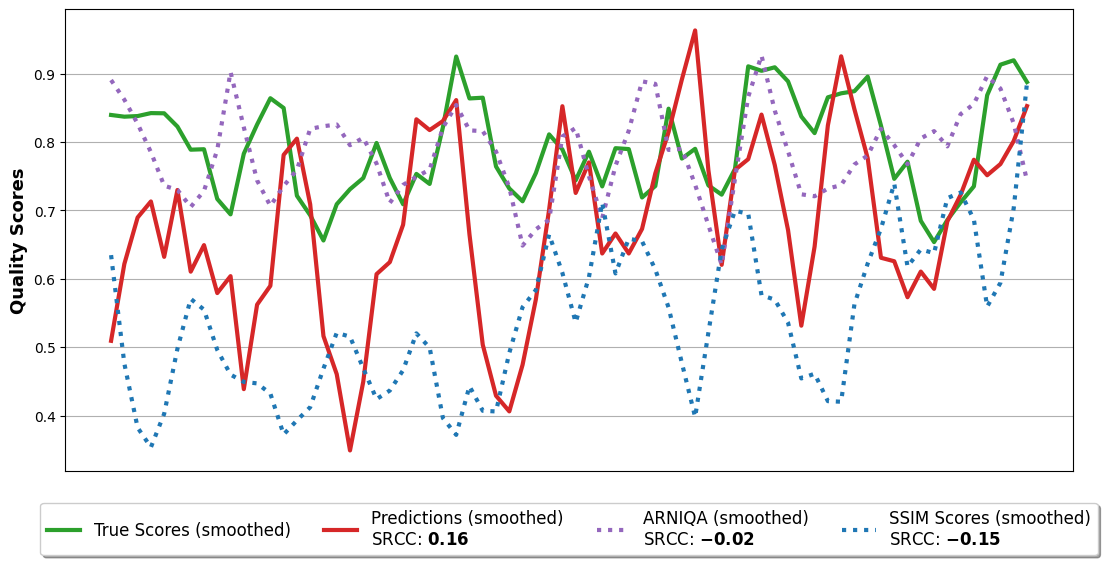
\includegraphics[keepaspectratio,width=15cm]{img/baseline_s2.png}
    \caption{Improved quality scores for synthetic distortion predictions with adjusted weights for less accurate quality criteria. The weights for field of view, orientation, and background were reduced, while the weights for focus, color calibration, and resolution were increased, resulting in an improved SRCC score.}
    \label{fig:BA2}
\end{figure}

\clearpage
\subsection{Out of Distribution Testing}
\label{sub:6}
In \autoref{fig:ood1}, images of animals, vehicles, and people were used to test the model’s performance on general images. The radar charts show that the model’s predictions for these images are quite accurate. This is because the model focuses on the types of distortions rather than the content of the image. For example, \autoref{fig:4l} and \autoref{fig:4ll} show the same image with different lighting distortions—one is brightened and the other is darkened. The model correctly spots these differences. Similarly, the good quality images in Figures \autoref{fig:3} and \autoref{fig:5} are also accurately predicted. \par
\vspace{\baselineskip}
\noindent
However, the model struggles with orientation and field of view distortions, which are more specific to teledermatology. This shows that while the model is not overfitted to teledermatology images, it is specially tuned to handle distortions important for this field. This means the model is flexible enough to work well on many types of images for common distortions but still needs improvement for specific teledermatology quality criteria. This balance makes sure the model is useful in many situations without losing its effectiveness for teledermatology. \par

\section{Key Model Assumptions and Their Implications}
\label{sec:KeyModelAssumptions}
The model assumes that the features extracted by ARNIQA’s backbone are detailed enough to identify the main distortions in teledermatology images. This assumption works well for lighting, focus, color calibration, and resolution, which cover four out of the seven dermatology quality criteria. However, the criteria for background, orientation, and field of view need more testing and adjustments. The current performance shows that the model is somewhat effective, and if the assumption that ARNIQA’s backbone can capture all key distortions is not entirely correct, it would mean that the model might not perform well in real-world scenarios where these distortions are common. To confirm these assumptions, more experiments with different datasets and real-world images should be conducted. By including a wider range of images in training, especially those with more background details, the model can be better prepared to handle real-world distortions. This is important for making the model stronger and more reliable in different situations. \par
\vspace{\baselineskip}
\noindent
Overall, the ARNIQA feature extraction backbone shows great potential for teledermatology applications, but continuous improvement and validation are essential to achieve the best possible performance. \par

\clearpage
\section{Reviewing the Objectives of the Thesis}
\label{sec:ReviewingObjectives}
At the beginning of this thesis, several specific objectives were outlined:

\begin{itemize}
    \item Conduct an extensive review of the literature on image quality assessment (IQA) methods, focusing on their application in teledermatology.
    \item Identify and select image quality metrics most suitable for assessing the quality of dermatological images.
    \item Evaluate the performance of selected image quality metrics on dermatological datasets to determine their effectiveness in assessing image quality.
    \item Develop a reproducible repository of image quality assessment tools and methodologies for teledermatology applications.
\end{itemize}
\noindent
The first objective was to perform a detailed review of the literature on image quality assessment methods and how they apply to teledermatology. This process took a lot of time but was very important for the rest of the work. Through this review, key concepts such as IQA, teledermatology,  and related studies were thoroughly examined and recorded. \par
\vspace{\baselineskip}
\noindent
The second objective was achieved during the literature review process. During this phase, the seven quality criteria from the International Skin Imaging Collaboration (ISIC) were found and chosen as the best metrics for assessing the quality of dermatological images. Selecting these dermatology quality criteria was very important for the next steps of the research. \par
\vspace{\baselineskip}
\noindent
For the third objective, the performance of the selected image quality metrics was evaluated on dermatological datasets. These evaluations were very detailed, involving tests on independent images that were not part of the model training. The datasets included both synthetically distorted images and images with real-world distortions, providing a complete assessment of how well the metrics worked. \par
\vspace{\baselineskip}
\noindent
The final objective was to develop a reproducible repository of image quality assessment tools and methods for teledermatology applications. This was successfully completed, creating a strong framework for future experiments and research. The repository makes sure that the methods and tools developed in this thesis can be used and built upon, helping further advancements in this field. \par

\clearpage
\section{Reflection}
\label{sec:Reflection}
This research showed that assessing image quality in teledermatology is possible with the proposed method, providing a good starting point for future studies. The research had both difficult and easier phases. Initially, understanding and connecting key concepts in teledermatology required a lot of reading and careful organization of information without losing sight of the main goals. These early challenges were important parts of the research process. Detailed records of these challenges and the steps taken to address them, as discussed in bi-weekly meetings, are included in \autoref{ch:Supplementary} for a complete overview. \par
\vspace{\baselineskip}
\noindent
Filtering good quality images and labeling the test set was the most time consuming and repetitive part of the research, but it was necessary. Accurate labeling ensured that model performance comparisons were reliable, and good quality images were crucial for effective training. While these task were tedious, their importance in achieving the research’s goals cannot be overstated. \par
\vspace{\baselineskip}
\noindent
Creating synthetic distortions and using severity ranges to generate artificial values for images was particularly interesting. Developing the distortion pipeline that could generate multiple synthetically distorted images from a single good quality image was one of the most innovative parts of this research. This new approach effectively addressed the lack of annotated images for teledermatology image quality assessment. By generating different distorted versions of the same image, the dataset was significantly expanded, which greatly improved the model’s performance. \par
\vspace{\baselineskip}
\noindent
The results showed that the model is robust and generalizes well, even when trained with a relatively small number of original images. The final model performed well, especially for criteria like lighting, focus, color calibration, and resolution. However, it still requires fine-tuning for field of view, background, and orientation distortions. Generally, high expectations are set, and leaving research unfinished is not preferred. However, due to time constraints, the research is complete up to this point. There remains potential for further improvements and more extensive testing to enhance the overall performance and reliability of the image quality assessment in the context of teledermatology. \par

\section{AI Tools Used}
\label{sec:AIToolsUsed}
In this work, several AI tools were used. ChatGPT was used to compress and summarize content. Additionally, it was used to optimize sentences and sections to make them more reader-friendly. Furthermore, GitHub Copilot was used in the development environment. It primarily helped in developing the Python scripts and models. These tools made the work more efficient and helped improve the overall quality of the thesis.


